\documentclass[12pt]{beamer}
\usetheme{sakura}
\usepackage{luatexja-ruby}
\ltjsetparameter{%
    jacharrange={%
        -2, % Exclude Greek and Cyrillic letters.
        -3  % Punctuations and Miscellaneous symbols.
    },
    alxspmode={`/,allow},
    alxspmode={`#,allow},
    alxspmode={92,allow}
}
\usepackage{fontawesome}
\iffontsavailable{HiraMaruPro-W4}{%
    \newjfontfamily\jtexttt{HiraMaruPro-W4}
}{%
    \newjfontfamily\jtexttt{some Japanese font}
}
\usepackage[sort]{natbib}
\usepackage{appendixnumberbeamer}
\usepackage{ccicons}
\usepackage{framed}
\usepackage{listings}
%https://tex.stackexchange.com/questions/24136/natbib-and-hyperref-for-author-year-style-produces-two-links/27235
\usepackage{etoolbox}
\usepackage{appendixnumberbeamer}

\makeatletter

\pretocmd{\NAT@citex}{%
  \let\NAT@hyper@\NAT@hyper@citex
  \def\NAT@postnote{#2}%
  \setcounter{NAT@total@cites}{0}%
  \setcounter{NAT@count@cites}{0}%
  \forcsvlist{\stepcounter{NAT@total@cites}\@gobble}{#3}}{}{}
\newcounter{NAT@total@cites}
\newcounter{NAT@count@cites}
\def\NAT@postnote{}

% include postnote and \citet closing bracket in hyperlink
\def\NAT@hyper@citex#1{%
  \stepcounter{NAT@count@cites}%
  \hyper@natlinkstart{\@citeb\@extra@b@citeb}#1%
  \ifnumequal{\value{NAT@count@cites}}{\value{NAT@total@cites}}
    {\ifNAT@swa\else\if*\NAT@postnote*\else%
     \NAT@cmt\NAT@postnote\global\def\NAT@postnote{}\fi\fi}{}%
  \ifNAT@swa\else\if\relax\NAT@date\relax
  \else\NAT@@close\global\let\NAT@nm\@empty\fi\fi% avoid compact citations
  \hyper@natlinkend}
\renewcommand\hyper@natlinkbreak[2]{#1}

% avoid extraneous postnotes, closing brackets
\patchcmd{\NAT@citex}
  {\ifNAT@swa\else\if*#2*\else\NAT@cmt#2\fi
   \if\relax\NAT@date\relax\else\NAT@@close\fi\fi}{}{}{}
\patchcmd{\NAT@citex}
  {\if\relax\NAT@date\relax\NAT@def@citea\else\NAT@def@citea@close\fi}
  {\if\relax\NAT@date\relax\NAT@def@citea\else\NAT@def@citea@space\fi}{}{}

\makeatother
\newenvironment{quoteblock}{%
    \def\FrameCommand{%
        {\color{sLightGray}{\vrule width 3pt}}%
        \hspace{10pt}
    }%
    \MakeFramed {\advance\hsize-\width \FrameRestore}}%
{\endMakeFramed}
\renewcommand\refname{参考文献}
\renewcommand\appendixname{付録}
\title{Lua\TeX{}-jaとbeamerで言語学関連のスライドを作る}
% \subtitle{副題}
\institute{総合研究大学院大学}
\author{宮澤 彬}
\date{{\number\year}年{\number\month}月{\number\day}日}
\hypersetup{%
    unicode,
    colorlinks,
    allcolors=sDarkBlue
}
\usepackage{gb4e,cgloss4e}
\noautomath%
\begin{document}

\begin{frame}[noframenumbering,plain]
    \nocite{demo}
    \maketitle
\end{frame}

\section{言語学関連}
\begin{frame}[fragile]
\frametitle{ギリシャ文字やキリル文字を使うときの注意点}
Lua\TeX{}-jaパッケージを読み込んだときに注意しなければならないのが,
ギリシャ文字やキリル文字を和文フォントが表示されることです.
プリアンブルに以下を追加して欧文フォントで表示されるようにしましょう.
\begin{leftbar}
% https://tex.stackexchange.com/questions/17774/listings-package-can-i-include-a-backslash-in-language-keyword-begin-for
\begin{lstlisting}[%
    language={[LaTeX]TeX},
    basicstyle=\ttfamily,
    % asterisk for highlight backslash
    texcsstyle=*\color{sRed}\bfseries,
    keywordstyle=\bfseries,
    moretexcs={ltjsetparameter},
    morekeywords={jacharrange},
    commentstyle=\color{sDarkBlue}
]
\ltjsetparameter{%
  jacharrange={%
    % Exclude Greek and Cyrillic letters
    -2,
    % Exclude Punctuations and Misc symbols
    -3
  }
}
\end{lstlisting}
\end{leftbar}
\end{frame}

\begin{frame}
\frametitle{あ}
    \begin{quoteblock}{\itshape
ἅπαν δὲ ὄνομά ἐστιν ἢ κύριον ἢ γλῶττα ἢ μεταφορὰ ἢ κόσμος ἢ πεποιημένον ἢ ἐπεκτεταμένον ἢ ὑφῃρημένον ἢ ἐξηλλαγμένον.}

\hfill アリストテレス「詩学」1457b
    \end{quoteblock}
\end{frame}

\subsection{例文と対訳}
\begin{frame}
\setlength{\glossglue}{5pt plus 2pt minus 1pt}\footnotesize
\frametitle{グロス}
\texttt{gb4e}と\texttt{cgloss4e}パッケージを使います.

\begin{exe}
    \ex%
    \glll%
    {これは} {ロシア語の} {教科書} {です} \\
    {\textit{kore-wa}} {\textit{rosia-go-no}} {\textit{kyōkašo}} {desu} \\
    {this-\textsc{top}} {Russia-language-\textsc{gen}} {textbook} {be} \\
    \trans%
    ``This is a textbook of the Russian language''
    \ex%
    \glll%
    {Это} {учебник} {русского} {языка} \\
    % {Э'то} {уче'бник} {ру'сского} {языка'} \\
    {\textit{èto}} {\textit{učebnik}} {\textit{russkovo}} {jazyka} \\
    {this} {textbook-\textsc{sg.nom}} {Russian-\textsc{m.sg.gen}} {language-\textsc{gen}} \\
    \trans%
    ``This is a textbook of the Russian language.''
\end{exe}
\end{frame}

\begin{frame}
    \frametitle{音声記号}
    Fira Sansフォントは多くの文字を含んでおり,またLua\LaTeX はユニコードによる入力に対応しているため,そのまま打ち込むだけで音声記号が表示されます.

    \smallskip

    (例)\textbf{медуза} [mʲɪˈduzə] くらげ

    \bigskip

    入力には以下を用いると便利です.
    \begin{itemize}
        \item Windows → \faGithub\ \href{https://github.com/samhocevar/wincompose}{\texttt{samhocevar/wincompose}}
        \item macOS → \faGithub\ \href{https://github.com/gnarf/osx-compose-key}{\texttt{gnarf/osx-compose-key}}
        \item Linux → 標準のCompose Key
    \end{itemize}
\end{frame}

\begin{frame}
    \frametitle{画像の引用}
    画像の挿入には\texttt{\textbackslash includegraphics}コマンドを使います.
    Creative Commonsライセンスの作品には\texttt{ccicons}パッケージのアイコンを利用すると便利です.
    必要に応じて\texttt{\textbackslash href\{}\emph{uri}\texttt{\}\{}\emph{text}\texttt{\}}で元のファイルへリンクを張ります.

    \bigskip

    \begin{figure}[b]
        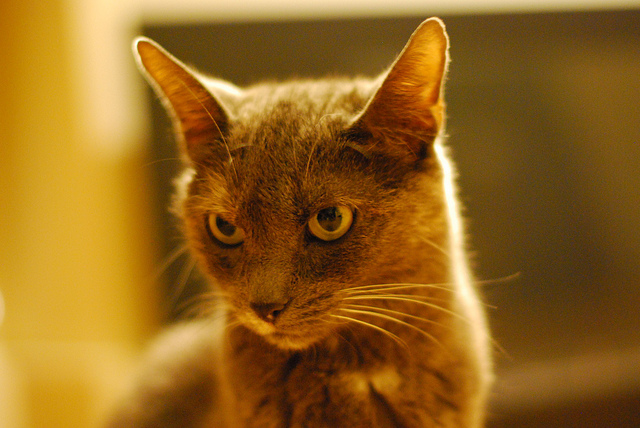
\includegraphics[width=0.4\textwidth]{cat.jpg}
        \caption{\href{https://www.flickr.com/photos/selda_eigler/8687127864/in/photolist-eeDNsC-qWFs4R-7CNDjJ-9c8DxY-eeDNhC-UCZ63T-dJNGUc-e5Nk39-988EVA-kUgwo-owDcVP-jQGjjt-5zkGTy-7WRCUo-b91XbZ-Mj8Ku-5pzwSA-9Bct2H-7CNHMY-7CJJMB-8MyEYn-9x45Mp-7JTq8M-ZrpGJ9-8fRht4-4SxVZT-5pzwjJ-ZsPJjL-aE44GL-dF6uWD-kqbHgM-5F373J-ZsQrVG-qyD7E9-ajyDPL-4WDvTp-KbDSc-5kCxD9-4MdeUo-pgDQcG-pPWrXD-662AFD-oTnC8k-apYceQ-nJSaaY-7CJLZv-7CJJMn-7CNFsU-XNMWkw-ccdtT9}{\emph{Cat} by Selda Eigler} \ccby.}
    \end{figure}

\end{frame}

\begin{frame}
    \frametitle{長め文章の引用}
    \begin{quoteblock}
        「あの森\ruby{琴}{ライラ}の宿でせう。
        あたしきつとあの森の中には、
        むかしの大きなオーケストラの人たちが集まつていらつしやると思ふわ。
        まはりには青い孔雀やなんかたくさんゐると思ふわ。」
        女の子が答へました。

        \hfill 宮澤賢治「銀河鉄道の夜」
    \end{quoteblock}
\end{frame}

\begin{frame}
\frametitle{参考文献の引用}
\texttt{{\textbackslash}citet\{key\}}で\citet{demo}のように地の文と同様の形式(textual)で引用されます.
一方\texttt{{\textbackslash}citep\{key\}}とすると丸括弧に入った形式(parenthetical)で引用されます\citep{demo}.
\end{frame}

\begin{frame}[plain,noframenumbering,allowframebreaks]
\frametitle{参考文献}
\footnotesize
\bibliographystyle{apalike}
\bibliography{demo}
\end{frame}

\appendix
\begin{frame}
    \footnotesize
    \frametitle{\appendixname}
    箇条書きの項目が鉤括弧から始まるときの注意点
    \begin{itemize}
        \item こんてちあ
        \item 「こんてちあ」

            行頭の余白が大きい
        \item \leavevmode\inhibitglue 「こんてちあ」

            \texttt{\textbackslash item \textbackslash leavevmode\textbackslash inhibitglue} で余白を調整
    \end{itemize}

    \bigskip

    参照:\href{http://doratex.hatenablog.jp/entry/20140714/1405302796}{TeX Live 2014のpTeX系列における\textbackslash inhibitglueの仕様変更}
\end{frame}


\end{document}
